\documentclass[../../main.tex]{subfiles}
\begin{document}

% Fluid simulation
% SPH 
% PCISPH
% Our contribution

%%%%%%%%
\section{Fluid simulation}
%%%%%%%%

In the field of computer graphics, realistic looking scenes and terrain has always been coveted. When it comes to fluid simulation there are multiple approaches to achieve realistic looking liquids. 
%With the increasing performance and memory capacity of computers, most areas are getting closer to being indistinguishable from reality. However, realistic looking fluid animation is still an area which is too computationally heavy to use efficiently(not implicit). There are multiple approaches with varying positive key aspects, they range in complexity from computationally expensive, high quality animations, towards simpler real-time systems. 




%Some kind of important-word list



Eulerian, or grid-based, methods are a common choice for simulating fluids in the industry due to high coherence with the ground reality. Physical quantities of the fluid are defined on a grid and they are then changed over time, but the grid remains fixed. This can be visualized as observing a river pass by while sitting at the riverbank, properties of constant points in the water change continuously, but the observed position is the same. 

Lagrangian methods, as opposed to the Eulerian, move fluid mass around explicitly. The quantities are tied to a small part of the fluid which is tracked through the whole simulation. An analogy would be sitting in a boat and drifting down a river while watching the water around the boat. These methods are usually more computationally expensive because parcel of fluid needs to be directly aware of its surroundings which requires expensive neighborhood calculations. On the other hand, they offer advantages on simulating small scale features like droplets and splashes because the surface is free and not bound to a grid. In addition, Lagrangian methods conserve mass implicitly and do not need a separate scheme for mass conservation. 

Whether a simulation is Eulerian or Lagrangian based, it is forwarded with a time step, a small value which is classically chosen globally and do not vary throughout the simulation. The time step determine how far the simulation is forwarded in each iteration. A higher time step decreases the required computational time but might also introduce stability concerns. Stability issues can occur when quantities in areas of the simulation are physically incorrect, such as the density being too high. It is, however, still desirable to have as high a time step as possible since while the real time simulated changes, the total computational time for each iteration stays the same. This means that more real time can be simulated with the same computational cost or that the same amount of real time can be simulated with less computational cost.


%%%%%%%%
\section{Smooth Particles Hydrodynamics}
%%%%%%%%
Our work is based on a variant of a Lagrangian method called Smooth Particles Hydrodynamics (SPH), as the name implies SPH uses particles to simulate fluids. Each particle uses the distance to its neighbours to calculate a density value, this value is then used to compute the forward force and velocity. The new position is calculated by forwarding every particle's current position a small distance, using its velocity and a given time step. 

It is important to make sure that particles do not end up inside each other after an iteration, as doing so would lead to undesirable visual effects. This limitation is called incompressibility and most liquids are approximated to be fully incompressible. The standard SPH method does not enforce incompressibility so in an attempt to do so, Becker and Teschner introduced Weakly Compressible SPH (WCSPH) \cite{becker2007weakly}. While this method enforced near-incompressibility it came with a time step restriction which made the simulation time quite long. (kan man använda quite?)

To increase the time step Solenthaler and Pajarola developed a Predictive-corrective Incompressible SPH (PCISPH) \cite{solenthaler2009predictive}. By using larger time step their approach could simulate further without the need of more computational power. This, however, introduced aforementioned errors in density, and thus made the entire simulation unstable. They solved this by introducing an additional step which predicts each particle's new position and iteratively applies a correction force if the density is over a certain threshold. The correction force is then used to calculate the particle's real new position. Although each iteration is more costly compared to WCSPH, a significant speedup is achieved because the time step can be many times larger. 

To further decrease computation time Solenthaler also introduced the Two-scale Resolution method \cite{}. This method uses two separate simulation with different particle sizes. The differently sized particles only interact with each other indirectly. One simulation uses larger (and therefore a smaller amount of) particles and the other simulation uses smaller particles but in a limited area. This area is usually only a subset of the scene where details are more important and therefore a speedup is achieved. 

In contrast to reducing the number of particles, Goswamis Regional Time Stepping \cite{} reduces computation time by using a time step based on the amount of movement in each area. Particles in calm areas gets a large time step and therefore updates less often, while in areas where there are collisions and lots of movement a smaller time step is used. 

Seeing as the two-scale resolution and regional time stepping methods improve on two different aspects of the PCISPH technique, we propose a method combining the two. Our method uses two simulations which calculates what time step to use in which regions individually. 

%\begin{figure}[h]
%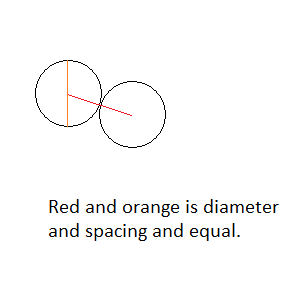
\includegraphics{image/spacing.png}
%\caption[Test image]{An image depicting the relationship between particle size and particle spacing.}     
%\label{fig:spacing}
%\end{figure}

%%%%%%%%
%\section{Methods for increasing performance}
%%%%%%%%
%{\color{red}\textit{Continuation on the SPH. Mention solutions for earlier mentioned problems.}}




\end{document}